\documentclass{report}
\usepackage[a4paper,margin=2cm]{geometry}
\usepackage{graphicx}
\usepackage{tikz}
\usepackage{lipsum}


% Définition des couleurs
\definecolor{bordercolor}{RGB}{0,0,0}
\definecolor{fillcolor}{RGB}{255,255,255}

% Commande pour encadrer le thème dans un rectangle
\newcommand{\framedtheme}[1]{%
  \begin{tikzpicture}
    \node[rectangle,draw=bordercolor,fill=fillcolor,inner sep=5pt] at (0,0) {\parbox{8cm}{\centering #1}};
  \end{tikzpicture}%
}

\begin{document}

\begin{titlepage}
  \begin{center}

    % Logo de l'université
    \includegraphics[width=4cm]{LogoU.png}

    \vspace{3cm}
    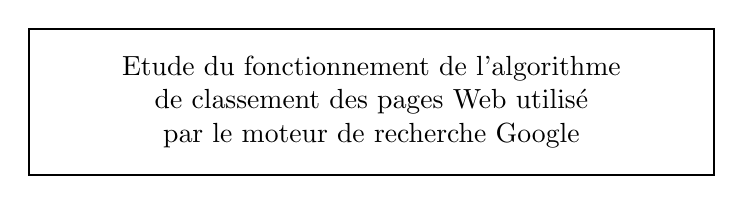
\begin{tikzpicture}
            \node[draw, thick, rectangle, inner sep=10pt, text width=8cm, align=center] 
            {Etude du fonctionnement de l’algorithme de classement des pages Web utilisé par le moteur de recherche Google};
        \end{tikzpicture}

    \vspace{1cm}

    % Noms des parties prenantes
    Présenté par : \\
    Nom de la Première Personne \\
    Nom de la Deuxième Personne \\
    Nom de la Troisième Personne

    \vspace{0.5cm}

    Encadré par : \\
    Nom de l'Encadreur

    \vfill

    % Date
    Date de soutenance

  \end{center}
\end{titlepage}

% Le reste du document

\end{document}
